\section{Judgments (Example Charts)}
Examples of judging a person's fortune and property primarily from the placement of the sect light's triplicity rulers.

\begin{figure}[H]
\centering
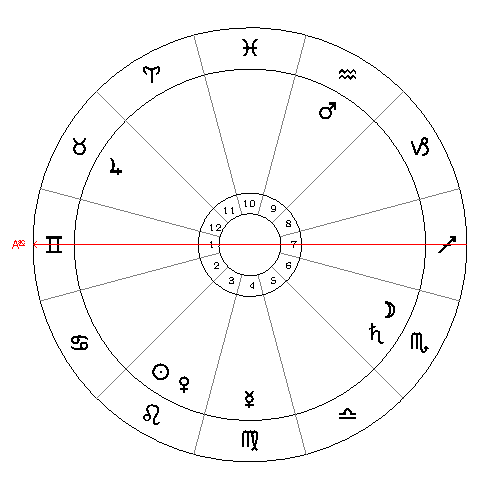
\includegraphics[width=0.7\textwidth]{charts/1_24_01}
\vspace{-1em}
\caption{Chart 02: Needy, Poor, Miserable}
\end{figure}

The nativity is nocturnal and the triplicity rulers of the \Moon\, in \Scorpio\, are first \Mars, second, \Venus. As both are cadent, ``this man should be needy, poor, not finding his daily bread, miserable. And this was in him more evident than what I told you.''

\begin{figure}[H]
\centering
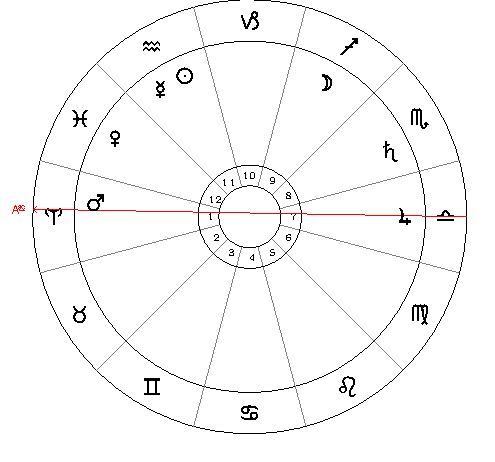
\includegraphics[width=0.7\textwidth]{charts/1_24_02}
\vspace{-1em}
\caption{Chart 03: Wealthy, Rich, Powerful}
\end{figure}

The nativity is diurnal and the triplicity rulers of the \Sun\, in \Aquarius\, are first, \Saturn, second, \Mercury; both in succedent places. \Mercury\, is in ``the place of fortune, so that the native should be wealthy, rich, powerful in business affairs, great in property, seizing eminence and fortune and increasing in them.''

\newpage
\begin{figure}[H]
\centering
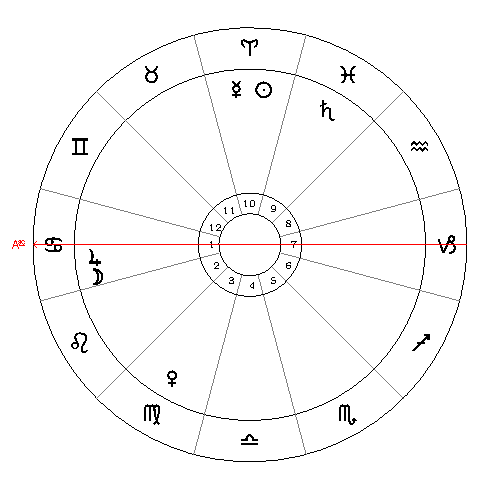
\includegraphics[width=0.7\textwidth]{charts/1_24_03}
\vspace{-1em}
\caption{Chart 04: Praised by kings, nobles, wealthy men}
\end{figure}

The nativity is diurnal\footnote{The position of \Mars\, was not given.} and the triplicity rulers of the \Sun\, in \Aries\, are, first, the \Sun, second, \Jupiter, both of which are in angles and in their own exaltations ``so that the native should be praised with the praise of kings and nobles and wealthy men.''

He will be ``praised with the praise of kings'' because \Saturn, the third triplicity ruler, is cadent in \Jupiter's sign (\Pisces) in trine to \Jupiter\footnote{\Saturn\, is in the 9th place which the Greeks associated with royalty.}.

\begin{figure}[H]
\centering
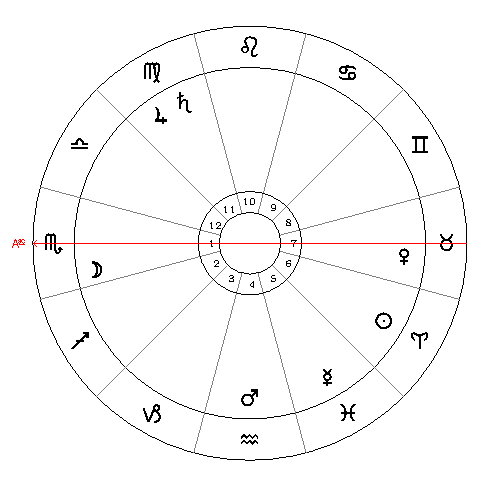
\includegraphics[width=0.7\textwidth]{charts/1_24_04}
\vspace{-1em}
\caption{Chart 04: Eminent, powerful, praised}
\end{figure}

The nativity is nocturnal and the triplicity rulers of the \Moon\, in \Scorpio\, are, first, \Mars, second, \Venus, third, the \Moon. As all three are angular ``this man is mighty in eminence, powerful in leadership so that crowns of gold and silver are placed on him and he is praised.''

\newpage
\begin{figure}[H]
\centering
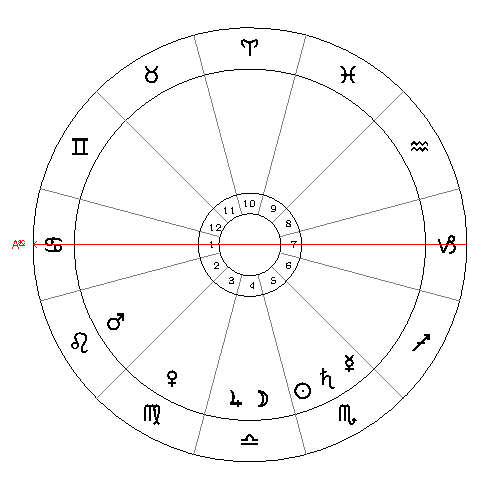
\includegraphics[width=0.7\textwidth]{charts/1_24_05}
\vspace{-1em}
\caption{Chart 05: Poor, unfortunate}
\end{figure}

The nativity is nocturnal and the triplicity rulers of the \Moon\, in \Libra\, are, first, \Mercury, second, \Saturn, third, \Jupiter. As the first and second rulers are cadent near the angle under the earth ``the man will be needy with respect to property'' but because the third ruler, \Jupiter, is with the \Moon\, in an angle ``he will have the closest thing to living out [his] days in poverty except that he will have the danger of the hand of misfortune.''\footnote{Dykes translates this as \textsl{``But because \Jupiter\, was in charge of some of this native, and he is with the \Moon\, in a stake, he will have the minimum of things, roughly what he is paid [with] daily, [but] having no importance [and] without a cessation of tribulation.'' (CAD 1.26.12)}}

\newpage
\begin{figure}[H]
\centering
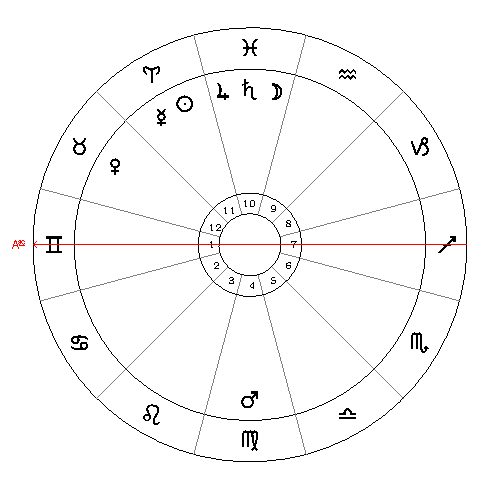
\includegraphics[width=0.7\textwidth]{charts/1_24_06}
\vspace{-1em}
\caption{Chart 06: Wealthy, an evil end}
\end{figure}

The nativity is diurnal and the triplicity rulers of the \Sun\, in \Aries\, are, first, the \Sun, second, \Jupiter, and third, \Saturn. As all three are in good places ``this man will abound in gold and silver'' but he will have an ``evil end'' because \Venus\, is the first triplicity ruler of the 4th ``from which the matter of the end and the situation of death are known'' and \Venus\,''is cadent in the sign of calamity\footnote{The 12th place.}.''

\newpage
\begin{figure}[H]
\centering
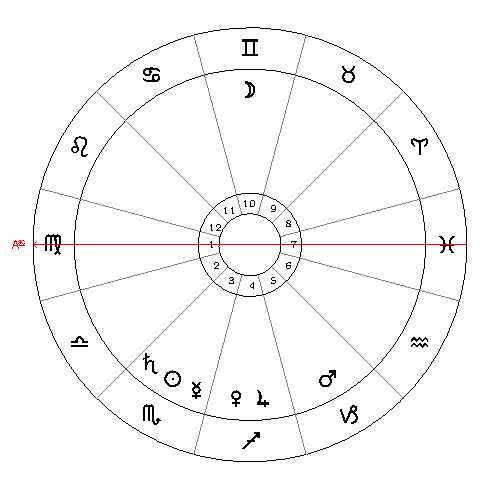
\includegraphics[width=0.7\textwidth]{charts/1_24_07}
\vspace{-1em}
\caption{Chart 07: Noble family but raised in poverty}
\end{figure}

The nativity is nocturnal and the triplicity rulers of the \Moon\, in \Gemini\, are, first, \Mercury, second, \Saturn, third, \Jupiter. The first and second are cadent, indicating ``poverty and indigence, and he will be beseeching all his days, but he will eat in misery...but since \Jupiter\, and \Venus\, are in cardines they indicate that he will be of noble lineage, but that he will be brought up and will grow up in houses of slavery, and he will curry favor with [his] brothers and nobles and will become acquainted [with them], but he will fail because of the evil effect of the lords of the \Moon's triplicity.''

\Mars\, ``indicates the loss of the property of his father and its dispersal in [all] directions''\footnote{Dykes, based on Pingree's timing for the chart, puts \Mars\, in the 2nd ``harming the native's assets'' but I believe the original also shows harm as \Mars, ruler of the 8th of inheritance in the 5th (risks) could indicate a sudden (\Mars\, exalted) loss (\Mars) of the father's assets (\Mars\, sextile \Saturn, \Sun) possibly due to his brothers (3rd) stealing them.}